%%%%%%%% ICML 2021 EXAMPLE LATEX SUBMISSION FILE %%%%%%%%%%%%%%%%%

\documentclass{article}

% Recommended, but optional, packages for figures and better typesetting:
\usepackage{microtype}
\usepackage{graphicx}
\iffalse
\usepackage{subfigure}
\fi
\usepackage{booktabs} % for professional tables
\IfFileExists{multirow.sty}{\usepackage{multirow}}{}
% hyperref makes hyperlinks in the resulting PDF.
% If your build breaks (sometimes temporarily if a hyperlink spans a page)
% please comment out the following usepackage line and replace
% \usepackage{icml2021} with \usepackage[nohyperref]{icml2021} above.
\usepackage{hyperref}
\hypersetup{hypertexnames=false}

\IfFileExists{caption.sty}{\usepackage{caption}}{}
\IfFileExists{subcaption.sty}{\usepackage{subcaption}}{}
\IfFileExists{listings.sty}{\usepackage{listings}}{}

% Attempt to make hyperref and algorithmic work together better:
\newcommand{\theHalgorithm}{\arabic{algorithm}}

\usepackage[accepted]{icml2021}
\usepackage[T1]{fontenc}
\let\tonOriginalTexttt\texttt
\renewrobustcmd{\texttt}[1]{%
\ifstrequal{#1}{experiments/hand\_detection\_recovery/plot\_results.py}%
{\tonOriginalTexttt{experiments/\allowbreak hand\_detection\_recovery/\allowbreak plot\_results.py}}%
{\tonOriginalTexttt{#1}}}


\makeatletter\let\tonTableInput\@@input\makeatother


% The Impact of Edge Detection on Sign Language Alphabet Recognition
\icmltitlerunning{Sign Language Alphabet Recognition}

\begin{document}

\pagenumbering{arabic}

\twocolumn[
\icmltitle{Sign Language Alphabet Recognition}

\begin{icmlauthorlist}
\icmlauthor{Ton Heijligers (852935308)}{ou}
\icmlauthor{Youri de Waal (852843968)}{ou}
\icmlauthor{Danny Linden (85261859)}{ou}
\end{icmlauthorlist}

\icmlaffiliation{ou}{Open Universiteit}
\icmlcorrespondingauthor{}{}

% You may provide any keywords that you
% find helpful for describing your paper; these are used to populate
% the "keywords" metadata in the PDF but will not be shown in the document
\icmlkeywords{}

\vskip 0.3in
]
\iffalse
\begin{abstract}
    Write a short abstract that contains a brief summary of the work and describes the main points you want to make.
    
\end{abstract}
\fi
\InputIfFileExists{ton_preview_notice.tex}{}{}



% Mijn idee is om te onderzoeken of we de inputafbeeldingen kunnen vereenvoudigen voordat we ze aan het model geven.
% We gebruiken een convolution/filter om vooral de randen met hoog contrast over te houden, zodat de vorm van de hand centraal staat en achtergrond, kleur en andere details grotendeels verdwijnen.
% Vervolgens trainen/testen we hetzelfde model op:
% 1. de originele afbeeldingen;
% 2. de vereenvoudigde edge-images.
% Onderzoeksvraag: Does edge-based image preprocessing improve sign language alphabet recognition?


\section{Brief Introduction}

We study ASL letter recognition from photographs through three changes: targeted data collection, detection recovery and hand-shape features. MediaPipe estimates 21 hand landmarks for classification \citep{ton-mediapipedocs,ton-shin2021}. Detection coverage and classification quality are evaluated separately. We use static A--Z images, without modelling the movements of J and Z.
\leavevmode \\\\
...
\\\
In the landmark-based recognition pipeline used in this study, hand landmark extraction determines which images can provide input to the letter classifier. When the detector returns \textit{no\_hand} landmarks, the image cannot be used for feature extraction and subsequent training. Improving detection coverage could therefore increase the number of images available for model training.
\\\\
In our baseline run on 78,000 ASL (American Sign Language) Alphabet training images covering the letters A-Z, MediaPipe returned \textit{no\_hand} detection for 17,598 images (22.56\%). A further 151 images produced multiple hand detections, while 60,251 images passed the single-hand acceptance criteria. These counts are reported in Section: \ref{sec:rq2-results} \nameref{sec:rq2-results} and can be reproduced from \texttt{baseline.csv} in the digital supplement for the \texttt{test\_all} run. These outcomes motivated an investigation of image preprocessing as a second detection attempt for initially missed images.
\\\\
We investigate a single application of morphological dilation using a square \(3 \times 3\) kernel, with erosion and a Canny-edge overlay included as comparison methods. 


%   Image N47 serves as a development example, followed by an evaluation on all initially missed A-Z training images. The same detector model and thresholds are used before and after preprocessing.
%   Because there are more than 17.000 images, we focussing on a specific image \ref{fig:N47_original} \nameref{fig:N47_original}.



\begin{enumerate}
    \item Does targeted data collection reduce confusion between certain letters more effectively than general data collection?
    \item To what extent does applying a \(3 \times 3\) dilation filter recover visually plausible hand landmarks in ASL Alphabet training images for which MediaPipe initially detects \textit{no\_hand}?
    \item Do explicit hand-shape categories and joint angles improve on, or replace, Shin's landmark directions?
\end{enumerate}

\section{Related works}
\iffalse
Briefly provide an overview of previous research and studies that are relevant to your topic. Show how this project fits into the broader conversation. Highlight what has already been done / discussed. Summarize key findings, identify gaps or limitations in existing research, and explain how your project builds on or differs from past efforts. Focus on the most important and credible sources and keep your explanations clear and concise.


\fi
Shin et al. describe ASL letters using distances and directions between estimated hand points \citep{ton-shin2021}. MediaPipe estimates 21 such points, including depth and a separate 3D world representation \citep{ton-mediapipedocs}. We examine whether explicit descriptions, such as a bent finger or two fingers being spread, add useful information to this representation. We distinguish the effect of adding features from the information a fitted model uses: permutation importance measures the latter and can be affected by related features \citep{ton-sklearnpermutation}.


\section{Methods}
\iffalse
Describe the methods used. How it works. It can include algorithms, system descriptions, new language constructs, analyses, etc.
Provide diagrams to help in the discussion. Figure \ref{fig:one-col-figure} and Figure \ref{fig:two-col-figure} shows an example of a one-column figure and a two-column figure. 


\fi
\subsection{Targeted training data (RQ1)}
We investigate whether additional training images reduce confusion between selected ASL letters. The original Kaggle predictions identify M/N and R/U as frequently confused pairs.

For the first experiment, the baseline is an existing 26-class SVM using 820 combined distance and direction features from Shin et al. (2021). A second model is retrained with the same configuration and original training data, supplemented by 60 new webcam recordings; 15 each of M, N, R and U.

To investigate whether the change in confusion can be attributed to additional samples for 1 letter alone, a third SVM classifier is trained, using the original development dataset, but supplemented with ONLY the 15 previously collected images for the letter N. All of the classifier parameters and 820-dimensional Shin feature representation remain unchanged. 

The N-only model is compared against the baseline and the previously retrained M/N/R/U model on the same 60 recorded test images. During this experiment, particular attention is given to the directional N-to-M and M-to-N confusion rates to determine whether improvements in N recognition introduce additional errors for M.
\subsection{Image Preprocessing}

For RQ2, image preprocessing is applied as a second attempt to obtain hand landmarks from images for which MediaPipe initially returns no hand detection. Three transformations are compared: dilation, erosion and a Canny-edge overlay. Each transformation modifies the original image independently, after which the same hand detector is applied again. This comparison measures whether changing the input image allows the detector to recover a previously missed hand.

    \subsubsection{Dilation}
        Replaces a pixel value in each color channel with the highest value in its vicinity. This allows light areas to expand and contours to change.

    \subsubsection{Erosion}
    	It uses the lowest value in that area. This allows light areas to become smaller and dark areas to expand.

    \subsubsection{Canny overlay}
        Zoekt randen op basis van veranderingen in helderheid en voegt de gevonden randen toe aan de oorspronkelijke kleurenfoto. In jouw implementatie worden die randen lichter gemaakt.


% \begin{figure*}
%     \centering
%     \includegraphics[width=\linewidth]{figures/example_pipeline.png}
%     \caption{One-column figure that explains the steps or framework of your method / model.}
%     \label{fig:two-col-figure}
% \end{figure*}


\par\noindent ...\par\medskip
\subsection{Hand-shape descriptions (RQ3)}\label{sec:ton-methods}
MediaPipe locates points on the hand, but the classifier needs numerical descriptions of their arrangement. Shin uses distances and directions between these landmarks. We ask whether explicit descriptions of finger shape add useful information, or can replace his directions.

We compare four feature blocks. Distances (D) describe how far landmarks are apart; Shin's directions (S) describe how the lines between them are oriented relative to the image axes. Our categories (E) describe recognizable properties, such as a bent finger, fingers being spread, or thumb position. Joint measurements (J) instead retain numerical angles at finger joints rather than assigning bending categories.

Keeping D and independently including or omitting S, E and J gives eight representations. We retrain both classifiers on each representation using the same fitting and test images. Comparing variants with and without E/J tests their added value; variants without S test whether they can replace Shin's directions. D/S use image landmarks, whereas E/J use estimated 3D world landmarks. A control also calculates J from Shin's image coordinates to examine this coordinate difference.

After training, we shuffle one feature group between held-out images without refitting. A score drop indicates model dependence on that group, which differs from the benefit of adding it during training \citep{ton-sklearnpermutation}. Definitions, settings and brief orientation follow-ups are in Appendix~\ref{app:ton-protocol}--\ref{app:ton-live}.

\par\noindent ...\par\medskip

\section{Experimental Results}
\subsection{Reducing letter confusion (RQ1)}
The Kaggle cross-validation results showed 119 M-to-N and 148 N-to-M errors, as well as 202 R-to-U and 40 U-to-R errors. These observations motivated the selection of M/N and R/U for targeted data collection.

On the seperately recorded test set, accuracy increased from 65.00\% to 78.33\% after retraining.
\begin{table}[ht]
\centering
\caption{RQ1: Paired evaluation on 60 test images.
Mutual confusion rates use 30 images per pair.}
\label{tab:rq1_results}
\begin{tabular}{lcc}
\toprule
Metric & Baseline & Retrained \\
\midrule
Accuracy & 65.00\% & 78.33\% \\
Macro-F1 & 0.6061 & 0.7758 \\
M/N confusion & 43.33\% & 23.33\% \\
R/U confusion & 26.67\% & 20.00\% \\
Correct predictions & 39/60 & 47/60 \\
\bottomrule
\end{tabular}
\end{table}

N-to-M errors decreased from 12 to 6, while R-to-U errors decreased from 8 to 6. The opposite error directions remained unchanged.

To investigate whether the reduction in M/N confusion could be attributed to additional N-examples alone, a third SVM was trained using the original dataset, but supplemented with ONLY 15 new N-images. All classifier settings and the 820-dimensional feature representation remained unchanged.

This N-only model was evaluated on the same 60 previously recorded test images as the baseline and four-letter extension.

\begin{table}[ht]
\centering
\caption{N-only comparison of training
conditions on the same 60 images.}
\label{tab:n_only}
\begin{tabular}{lccc}
\toprule
Metric & Base & N-only & MNRU \\
\midrule
Accuracy (\%) & 65.0 & 73.3 & 78.3 \\
M $\rightarrow$ N & 1 & 2 & 1 \\
N $\rightarrow$ M & 12 & 6 & 6 \\
R $\rightarrow$ U & 8 & 8 & 6 \\
M/N confusion (\%) & 43.3 & 26.7 & 23.3 \\
\bottomrule
\end{tabular}
\end{table}

Adding only N-examples reduced N-to-M misclassifications from 12 to 6. However, M-to-N errors increased from 1 to 2, indicating a possible trade-off between recognition of the two letters. Dispite this increase, overall M/N confusion decreased from 43.3\% to 26.7\%. The four-letter extension achieved a slightly lower M/N confusion rate of 23.3\%.
    \subsection{Datasets}
        \iffalse
Include a description of the data used, what it contains, train test splits, etc.
\fi
For RQ3, classification uses only the 60,251 original images with an accepted single-hand detection; missing detections are excluded. Five fixed folds separate blocks of consecutive file numbers. These blocks are not verified participants. Every representation uses the same held-out sources, and every image receives one out-of-fold prediction. Recovered images from RQ2 are not added to this feature comparison. Its scores therefore describe classification after accepted detection, rather than the full recognition pipeline.

\leavevmode 
        \\\\
        ...
        \\\\
        
        For RQ2, we use the A-Z training images from the Kaggle ASL Alphabet dataset. This subset contains 78,000 images, with 3,000 images per letter. The additional classes \textit{space}, \textit{delete}, and \textit{nothing} are outside the scope of this experiment.
        \\\\
        All original images are first processed by MediaPipe. Images with the status \texttt{no\_hand} are selected for the recovery experiment. The supplied Kaggle test images are excluded from RQ2. This experiment evaluates hand-detection recovery within the original training images.
        \\\\
        Image N47 (Figure~\ref{fig:N47_original}) is used as a development example to inspect the effect of dilation. The complete evaluation includes N47 and images inspected during earlier development. It therefore describes the results on the full dataset, including previously examined images.
        
    \subsection{Implementation Details}
The feature comparison trains eight representations with two learners across five folds: 80 models. Model settings remain fixed across representations. Only J is imputed and standardized, using the training fold. We report macro-precision and macro-F1 over A--Z, giving each letter equal weight. A paired comparison counts corrected and newly introduced errors on the same images. Appendix~\ref{app:ton-protocol} gives the settings, feature dimensions and reproducible result paths.

\leavevmode 
        \\\\
        ...
        \\\\
        
        MediaPipe Hand Landmarker processes each image in IMAGE mode, with both detection and presence thresholds set to 0.50. Up to two hands are detected so that multiple-hand outputs can be identified. The same model and settings are used for the original and processed images.\footnote{The detector configuration and output validation are implemented in \texttt{research/data.py}, in the \texttt{Detector} class.} The software versions, settings and checksums are recorded in \texttt{\ref{fig:preprocessing-config} settings.json} in the digital supplement for the \texttt{test\_all} run.
        \\\\
        Each image with the original status \texttt{no\_hand} is processed using three separate variants. Dilation and erosion each use a square $3 \times 3$ kernel with one iteration. Both operations are applied to the colour image at its original resolution.
        \\\\
        For the Canny-overlay variant, the image is converted to grayscale and smoothed using a $5 \times 5$ Gaussian filter. Canny edge detection uses thresholds of 50 and 150. The resulting edge map is converted to three channels and added to the original colour image, using weights of 0.25 for the edges and 1.0 for the original image.
        \\\\
        Each variant is created independently from the original image. The processed images are saved as lossless PNG files and passed to the same detector during the retry step.\footnote{The transformations are defined in the \texttt{variants} function in \texttt{research/morphology\_pilot.py}. The baseline, preprocessing and retry stages are implemented in \texttt{research/recovery\_experiment.py}.}
        \\\\
        Outputs are paired using the original image identifier. Technical recovery is defined as a transition from \texttt{no\_hand} to \texttt{ok}, requiring exactly one detected hand and successful geometric validation. For the combined result, each image is counted once if at least one variant produces \texttt{ok}. A systematic visual assessment of the recovered landmarks remains to be completed.
        \\\\
        The exported results are analysed using pandas to calculate recovery counts and percentages per preprocessing variant and per letter. Each recovery percentage uses the number of originally missed images in the corresponding group as its denominator. An image may contribute to multiple variant counts, while the combined recovery count includes each image only once.
        \\\\
        Matplotlib is used to visualise the results calculated with pandas. The figures are exported as PNG and PDF files. The underlying plotting data are saved as CSV files, together with source-file checksums and plotting-library versions, to support verification and reproduction.\footnote{The calculations and figures are generated by \texttt{experiments/hand\_detection\_recovery/plot\_results.py}.}
        
    
    \subsection{Results}
    \label{sec:rq2-results}
\iffalse
        Analyze and discuss your results. Table \ref{tab:example-table} shows an example of a table.
        Include plots and visualizations such as Figure \ref{fig:one-col-figure}.

\fi
\paragraph{RQ3: feature comparison.}
Table~\ref{tab:ton-features} compares all eight descriptions. With Shin as the SVM baseline, our categories lose 22 correct predictions; world-joint angles gain 67, and both additions together lose three. The same-coordinate angle control gains only four. The larger world-angle gain therefore cannot be attributed to the angle formula alone. The small SVM improvement does not recur with LightGBM.

\begin{table*}[t]\centering\small
\caption{RQ3: pooled classification on 60,251 accepted original images. D: distances; S: directions; E: own categories; J: world-joint measurements. P is macro-precision (\%). All variants contain D.}
\label{tab:ton-features}
\begin{tabular}{lrrrr}\toprule
 & \multicolumn{2}{c}{SVM} & \multicolumn{2}{c}{LightGBM}\\
Hand description & P & F1 & P & F1\\\midrule
\tonTableInput ton_feature_rows_en.tex
\bottomrule\end{tabular}
\end{table*}

In the models with D/S/E, shuffling thumb flexion produces the largest mean F1 drop among our categories for SVM (0.08 percentage points); for LightGBM it is middle--ring spreading (0.03). This identifies model dependence, rather than a guaranteed benefit from adding a feature.

\paragraph{Brief practical explorations.}
Alongside the feature study, we briefly tried ideas for left/right handling and G/H camera views. Mirror training and right normalization help on artificial mirror tests but lose 26 and 136 correct predictions on originals. G/H rotation learns the offered artificial geometry, while two selected live G examples remain H. These small exploratory checks do not establish better recognition for new users; protocols, scores and examples are in Appendix~\ref{app:ton-orientation}--\ref{app:ton-live}.


\par\noindent ...\par\medskip
        In the baseline run, 60,251 of the 78,000 A-Z training images passed the single-hand acceptance criteria. MediaPipe returned \textit{no\_hand} detection for 17,598 images (22.56\%) and multiple hands for 151 images (0.19\%). The complete per-image detection results are available in \texttt{baseline.csv} in the digital supplement for the \texttt{test\_all} run.
        \\\\
        For the development example N47, the original image produced \textit{no\_hand} detection. After one application of $3 \times 3$ dilation, the detector returned one hand that passed geometric validation under the same confidence thresholds. The measured outcomes for this image are recorded in \texttt{n47\_example.csv}.
        \\\\
        All 17,598 initially missed images were subsequently processed using the three variants. Dilation recovered 3,560 images (20.23\%), erosion recovered 2,018 images (11.47\%), and the Canny overlay recovered 1,391 images (7.90\%). At least one variant recovered 4,799 unique images (27.27\%). Figure~\ref{fig:rq2-recovery} compares the individual recovery rates with the combined result.


        
        \begin{figure*}[h]
            \centering
            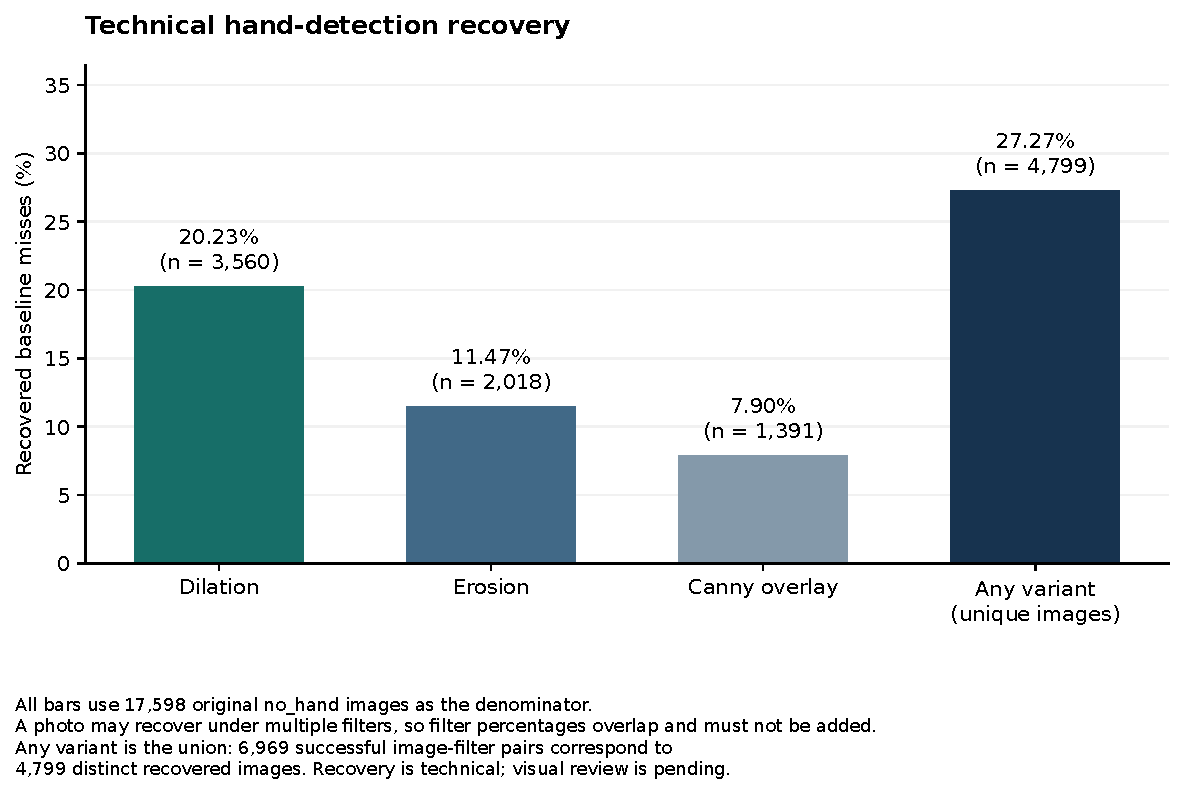
\includegraphics[width=\linewidth/2]{figures/recovery_by_variant.pdf}
            \caption{Technical recovery among the 17,598 originally missed images. Individual filter groups overlap because an image can be recovered by multiple variants. The combined result counts each recovered image once. Percentages were calculated using pandas and plotted with Matplotlib.}
            \label{fig:rq2-recovery}
        \end{figure*}
        
        The percentages for the individual variants overlap. An image recovered by both dilation and erosion contributes to both variant counts, but only once to the combined result. The three variants produced 6,969 successful image-filter pairs, corresponding to 4,799 distinct recovered images. The individual percentages therefore cannot be added to obtain the combined recovery percentage.
        \\\\
        Of the 4,799 recovered images, 3,024 were recovered by exactly one variant, 1,380 by exactly two variants, and 395 by all three variants. These counts explain the difference between the total number of successful image-filter pairs and the number of unique recovered images.
        \\\\
        After all retries, 12,799 images had no accepted detection under any variant. Of these, 12,779 images retained the status \texttt{no\_hand} under all three variants. The remaining 20 images produced another rejection status under at least one variant.
        \\\\
        The per-image outcomes and successful variants are recorded in \texttt{per\_image.csv}. Images without an accepted retry are listed in \texttt{unrecovered.csv}. Images with \texttt{no\_hand} under every variant are listed separately in \texttt{still\_no\_hand.csv}. These results quantify technical recovery. The proportion of visually plausible recoveries has not yet been established.
        \\\\
        To assess repeatability, the complete experiment was executed a second time on the same workstation using identical recorded settings, software versions and model files. Both runs produced identical detection outcomes for all 78,000 original images and identical checksums for all 52,794 processed images. The retry statuses also matched for every image and variant. For all 6,969 successful retries, the stored image and world landmark coordinates were exactly equal. Both runs recovered 4,799 unique images, corresponding to 27.27\% of the originally missed images. The comparison results and checksums of the compared output files are recorded in \texttt{\ref{fig:repeatablity} \nameref{fig:repeatablity}} in the digital supplement for the \texttt{test\_all\_repeat} run.
        
    \subsection{Discussion}
\iffalse
        Additionally, you can include a separate discussion section in which you summarize the results, indicate possible limitations of your work, and provide suggestions for future research.

\fi
\paragraph{RQ1: interpretation and limitations.}
The results suggest that additional training examples can improve recognition of selected frequently confused letters. In particular, recognition of N improved considerably without reducing recognition of M on the evaluated images. 

However, the additional training and test images were collected from the same person. Although the sessions were separate, this does not establish generalization. Also, only four of the 26 ASL letters were evaluated. Other potential effects on unevaluated letters remain unknown. The findings should be interpreted as a small-scale, single-participant evaluation rather than a general performance guarantee.
\par\noindent ...\par\medskip
\paragraph{RQ3: interpretation and limitations.}
Our categories do not consistently improve on Shin, and categories plus joint angles do not fully replace his directions under the tested settings. The small world-angle improvement depends on the learner and coordinate source. Permutation dependence should not be read as the gain from adding a feature.

The short left/right and G/H explorations illustrate limits of synthetic changes: improved artificial scores do not establish better live recognition. They are practical follow-ups, not additional independent validation of the main feature study. Rigid G/H rotation preserves geometry and does not recreate new detector errors under occlusion.

The folds were inspected during development and are not verified people, so these are exploratory results rather than an untouched final test. Detection recovery, accepted-image classification and selected webcam errors have different denominators and should be interpreted separately.


\par\noindent ...\par\medskip
        Dilation produced the highest technical recovery rate of the three evaluated variants. The higher combined recovery rate shows that the other variants also recovered images that dilation did not recover. However, the combined result requires trying all three variants and accepting an image when at least one attempt succeeds.
        \\\\
        The N47 example demonstrates that a small change to the input pixels can change the detection outcome while the model and thresholds remain fixed. The experiment does not establish which individual change in a contour, texture or contrast caused this response. Such explanations require further controlled comparisons and visual inspection.
        \\\\
        The results are limited to the evaluated dataset and detector configuration. N47 and earlier development images are included in the complete run, and the reported results therefore include previously examined examples. In addition, technical recovery does not establish the accuracy of the estimated hand points. A visual assessment is needed to determine whether the recovered landmarks are plausible.
        \\\\
        The agreement between the two runs supports repeatability under the recorded conditions. Repeatability across other computers, software versions or detector models was not evaluated. The coordinate comparison covers the retry detections, as landmark coordinates from the original baseline images were not retained.
        \\\\
        The contribution to RQ2 is therefore the measured technical recovery of initially missed images. Whether these recovered images improve letter recognition requires a separate training and evaluation experiment.
        
\iffalse
    \subsection{Citing references}
        LaTeX manages the citations for you. You simply have to add the bibtex entry for the reference in the references.bib file and you can use the citation in the paper \cite{langley00}. You can also cite multiple references in one command \cite{DudaHart2nd,Newell81,kearns89}. The bibtex entries for a paper can be obtained in websites such as google scholar or dblp.
        
        \begin{table}[h]
            \centering
            \label{tab:example-table}
            \caption{Example Table}
            \begin{tabular}{lllll}
                \toprule
                \multirow{2}{*}{Models} & \multicolumn{3}{c}{Metric 1} & Metric 2\\
                \cmidrule{2-4} \cmidrule{5-5} \\
                {} & precision & recall & F-score  & R@10 \\
                \midrule
                model 1 & 0.67  & 0.8 & 0.729  & 0.75 \\
                model 2 & 0.8 & 0.9 & 0.847 & 0.85 \\
                \bottomrule
            \end{tabular}
        \end{table}


\fi
\IfFileExists{references.bib}{\bibliography{references,ton_references}}{\bibliography{ton_references}}
\bibliographystyle{icml2021}


\clearpage
\onecolumn
\appendix
\section{Appendices}



\begingroup
\let\verbatim\relax
\let\endverbatim\relax
\lstnewenvironment{verbatim}{\lstset{basicstyle=\ttfamily\scriptsize,breaklines=true,breakatwhitespace=false,columns=fullflexible,keepspaces=true,showstringspaces=false}}{}
\begin{figure}[H]
\centering
\begin{minipage}{0.95\linewidth}
\begin{verbatim}
{
  "source": "...ktai-hand-gesture\\data
            \\asl-alphabet-download",
  "limit": null,
  "inventory_sha256": "...",
  "images": 78000,
  "mediapipe": "0.10.35",
  "opencv": "4.14.0",
  "detector_sha256": "...",
  "detection_confidence": 0.5,
  "presence_confidence": 0.5,
  "num_hands": 2,
  "mode": "IMAGE",
  "kernel": [ 3, 3 ],
  "iterations": 1,
  "canny_thresholds": [ 50, 150 ],
  "blur": [ 5, 5 ],
  "overlay_weights": [ 1.0, 0.25 ],
  "code_hashes": {
    "data.py": "...",
    "morphology_pilot.py": "...",
    "recovery_experiment.py": "..."
  }
}
\end{verbatim}
\end{minipage}
\caption{Configuration of the image preprocessing pipeline}
\label{fig:preprocessing-config}
\end{figure}
\begin{figure}[H]\centering
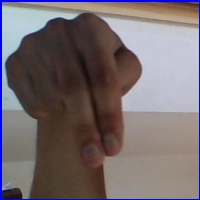
\includegraphics[height=30mm]{figures/N47_original.png}\hspace{8mm}
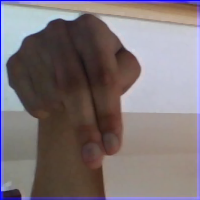
\includegraphics[height=30mm]{figures/N47_dilated.png}\hspace{8mm}
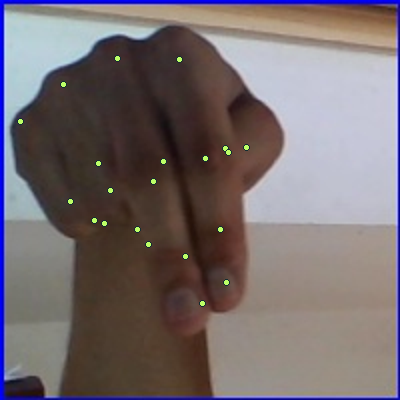
\includegraphics[height=30mm]{figures/N47_overlay.png}
\caption{N47 in its original form (left), after dilation (centre), and with recovered points overlaid on the original pixels (right). The overlay supports inspection; it does not constitute an independent landmark accuracy assessment.}
\label{fig:rq2-n47}\label{fig:N47_original}
\end{figure}

\clearpage
\begin{figure}[H]
\centering
\begin{minipage}{0.95\linewidth}
\begin{verbatim}
{
  "reference": "ktai-hand-gesture\\experiments\\hand_detection_recovery\\runs\\test_all",
  "repeat": "ktai-hand-gesture\\experiments\\hand_detection_recovery\\runs\\test_all_repeat",
  "settings_equal": true,
  "changed_settings": [],
  "baseline": {
    "reference_records": 78000,
    "repeat_records": 78000,
    "different_records": 0
  },
  "processed": {
    "reference_records": 52794,
    "repeat_records": 52794,
    "different_records": 0
  },
  "retry": {
    "reference_records": 17598,
    "repeat_records": 17598,
    "different_records": 0
  },
  "summary": {
    "reference_records": 4,
    "repeat_records": 4,
    "different_records": 0
  },
  "landmarks": {
    "reference_records": 52794,
    "repeat_records": 52794,
    "records_with_coordinates": 6969,
    "different_coordinate_records": 0,
    "different_metadata_records": 0,
    "maximum_absolute_coordinate_difference": 0.0
  },
  "all_compared_outputs_equal": true,
  "evidence_sha256": {
    "reference": {
      "settings.json": "748dbe1997f11e793ef067d48342281f3a768e403a26d301f44cdc9b790a6e07",
      "baseline.csv": "2844e86d3309cc6ce6ca2915000f71b0a850e9ef8f17e42210a2b8dc766cd4c3",
      "processed.csv": "87805980df2d78ae7a2144120f01ba4a14542fc3b50a0ada4545947e8d790595",
      "per_image.csv": "79da23909a82dab478037b5f3c516a79c0d6591c0806f810f996ea18227e11e4",
      "summary.csv": "4c312ec4f3e4bb884c6e15f86dcef997815fa66f9642dda124b1d62c2315d556",
      "retry_landmarks.jsonl": "84e1273caba566c398ee1c833d5a0f7eb4ea087d2d87be459c2379c2c4457394"
    },
    "repeat": {
      "settings.json": "748dbe1997f11e793ef067d48342281f3a768e403a26d301f44cdc9b790a6e07",
      "baseline.csv": "2844e86d3309cc6ce6ca2915000f71b0a850e9ef8f17e42210a2b8dc766cd4c3",
      "processed.csv": "55c8c232a27aedac7344fec9b11eef80f76c4e2ee764f45b2c8aa5d6d98ae1f8",
      "per_image.csv": "79da23909a82dab478037b5f3c516a79c0d6591c0806f810f996ea18227e11e4",
      "summary.csv": "4c312ec4f3e4bb884c6e15f86dcef997815fa66f9642dda124b1d62c2315d556",
      "retry_landmarks.jsonl": "41513daca93729e615f589fc20c04def71e610176dfd8dc135cb782cd695f502"
    }
  },
  "scope": "Two executions on the same workstation. Baseline coordinates were not exported; coordinate comparison covers retry detections. Absolute output paths are excluded from content comparisons."
}
\end{verbatim}
\end{minipage}
\caption{Configuration of the image preprocessing pipeline}
\label{fig:repeatablity}
\end{figure}
\endgroup

%\subsection{Exploratory preprocessing experiments for RQ1}
...
\\\
...
\\\
...
\\\
...


%\subsection{Exploratory preprocessing experiments for RQ2}
\label{app:rq2-pilot}

\subsubsection{Provenance and purpose}
The experiments documented here were implemented and executed by the Codex assistant during the project discussion, using the locally available Kaggle ASL Alphabet images. The assistant added the baseline and pilot scripts and ran the measurements. Student reproduction and the planned visual assessment remain outstanding. These results document the development of the proposed dilation experiment.

RQ2 concerns recovery of visually plausible hand landmarks among initially missed images. The measurements below establish technical recovery. The visual plausibility of all recovered configurations has yet to be assessed using a fixed rubric. N47 and other inspected pilot images should be identified as development data when constructing a subsequent evaluation set.

\subsubsection{Fresh baseline and training}
The baseline processed 78,000 original A--Z training images, comprising 3,000 images per letter. The additional classes were excluded. MediaPipe Hand Landmarker 0.10.35 ran in IMAGE mode, with a maximum of two hands and detection and presence thresholds both set to 0.50. The model file was \texttt{models/hand\_landmarker.task}. A result received \texttt{ok} when exactly one hand was returned and the project's geometric validation passed.

\begin{table}[ht]\centering
\caption{Fresh detection outcomes on original A--Z training images.}
\label{tab:rq2-baseline}
\begin{tabular}{lrr}\toprule
Outcome & Images & Percentage\\\midrule
One valid hand (\texttt{ok}) & 60,251 & 77.245\\
Zero hands (\texttt{no\_hand}) & 17,598 & 22.562\\
Multiple hands & 151 & 0.194\\
Invalid geometry & 0 & 0.000\\\midrule
Total & 78,000 & 100.000\\\bottomrule
\end{tabular}
\end{table}

A fresh SVM letter classifier was fitted to the 60,251 accepted images using 820 Shin descriptors and 15 angle features. This produced \texttt{runs/clean\_training/asl\_clean.joblib}. Its fit has no independent test score. The recovery experiments below use the pretrained MediaPipe detector; the letter classifier does not determine whether a hand is detected.

\subsubsection{N47 development example}
The original N47 image returned \texttt{no\_hand}. One application of dilation with a square \(3\times3\) kernel changed its output to \texttt{ok} at the same detector thresholds. Erosion and the tested Canny overlay retained \texttt{no\_hand}. In separate threshold probes on the original pixels, lowering only the detection threshold to 0.49 retained \texttt{no\_hand}, while 0.45 yielded \texttt{ok}. These probes show sensitivity to both preprocessing and threshold choice.

The initial N47 probes were executed as terminal commands, and their outputs were recorded in the conversation. They were not exported as a dedicated CSV. The original-versus-dilation transition was subsequently rerun when generating the example images below. The exact internal detection score was not recorded.

\begin{figure}[ht]\centering
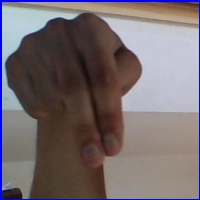
\includegraphics[height=30mm]{figures/N47_original.png}\hspace{8mm}
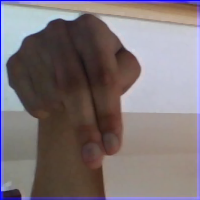
\includegraphics[height=30mm]{figures/N47_dilated.png}\hspace{8mm}
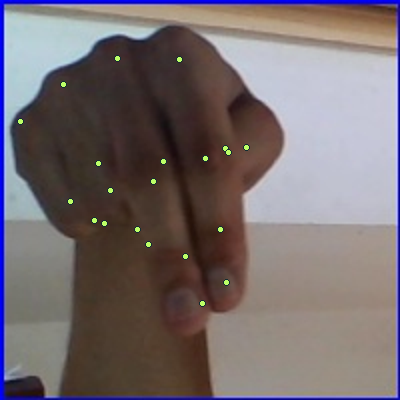
\includegraphics[height=30mm]{figures/N47_overlay.png}
\caption{N47 in its original form (left), after dilation (centre), and with recovered points overlaid on the original pixels (right). The overlay supports inspection; it does not constitute an independent landmark accuracy assessment.}
\label{fig:rq2-n47}
\end{figure}

\clearpage
\subsubsection{Letter-balanced pilot}
Using random seed 42, the pilot selected 20 initially missed and 10 initially accepted images per letter, giving 520 misses and 260 controls. The original status was rechecked before applying each transformation. Every selected photo received each of the three transformations below, with fixed detector settings.

\begin{itemize}
\item Dilation used \texttt{cv2.dilate} with a \(3\times3\) square kernel and one iteration.
\item Erosion used \texttt{cv2.erode} with the same kernel and iteration count.
\item The Canny overlay used a grayscale conversion, a \(5\times5\) Gaussian blur and Canny thresholds of 50 and 150. The three-channel edge map was added to the original RGB image with weights 0.25 and 1.0, respectively.
\end{itemize}

Image dimensions were retained, and processed arrays were supplied directly to the detector. Technical recovery means a transition from \texttt{no\_hand} to \texttt{ok}. Control loss means that an originally accepted image no longer received \texttt{ok}.

\begin{table}[ht]\centering
\caption{Exploratory pilot outcomes. Recovery denominators are 520 misses; loss denominators are 260 controls.}
\label{tab:rq2-pilot}
\begin{tabular}{lrrrr}\toprule
Transf. & Recovery & Rec (\%) & CL \footnote{Control losses} & Loss (\%)\\\midrule
Dilation & 130 & 25.00 & 6 & 2.31\\
Erosion & 64 & 12.31 & 8 & 3.08\\
Canny overlay & 49 & 9.42 & 28 & 10.77\\\bottomrule
\end{tabular}
\end{table}

The pilot gave equal weight to each letter, whereas the complete set of missed images has unequal letter counts. Its recovery percentage therefore does not directly estimate recovery across all 17,598 misses. Control losses describe applying preprocessing to already accepted images. A second-attempt procedure restricted to baseline misses bypasses these controls.

\subsubsection{Code and retained evidence}
All paths below are relative to the project root containing \texttt{app.py}.
\begin{itemize}
\item \texttt{research/data.py}, class \texttt{Detector}, defines detector settings and geometric validation.
\item \texttt{research/clean\_training.py} runs the baseline and prepares accepted inputs. The fresh classifier fit uses \texttt{--fresh-fit} in \texttt{research/live\_model.py}.
\item \texttt{research/morphology\_pilot.py} contains the transformations, deterministic sampling, paired comparisons and pilot exports.
\item \texttt{runs/clean\_training/all\_images.csv}, \texttt{no\_hand.csv} and \texttt{by\_letter.csv} contain the baseline inventory and summaries.
\item The pilot directory is \texttt{runs/clean\_training/morphology\_pilot/}. It contains \texttt{per\_foto.csv} with paired outcomes, \texttt{summary.csv} with aggregate results and \texttt{controle\_*.jpg} with overlays of recovered detections.
\end{itemize}

The pilot exports status changes and rendered overlays. A separate numerical export of all recovered landmark coordinates and a completed visual-review dataset are not yet available. The earlier \texttt{historical\_image\_audit.py} reconstructed membership in the historical accepted cohort by image ID. The fresh detector outputs listed above are the source for the present baseline counts.

\subsubsection{Reproduction and next measurement}
Run \texttt{python -m research.clean\_training --out runs/clean\_training}
from the project root with the configured Python environment. The command requires a new output directory. The existing baseline can be used to rerun \texttt{python -m research.morphology\_pilot}; this command writes to the existing pilot output paths. Preserve the original evidence before rerunning it.

A subsequent study should freeze the transformation and visual rubric, identify the development-image exclusions, and report technical and visually plausible recovery with the same eligible-image denominator. The exploratory outcomes in this appendix can motivate that design.


%\subsection{Exploratory preprocessing experiments for RQ30}
...
\\\
...
\\\
...
\\\
...




\par\noindent ...\par\medskip
\clearpage
\onecolumn
\section{RQ3: feature definitions and evaluation}\label{app:ton-protocol}
This supplement gives the feature definitions, evaluation protocol and separate orientation controls supporting RQ3.

\subsection{Source selection, folds and model settings}
The feature study uses 60,251 accepted original A--Z images. The original Kaggle test images duplicate training sources and are not used as an independent test. Five frozen folds separate six blocks of consecutive file numbers, not verified participants. Every representation shares source IDs, labels and held-out partitions. Test folds were inspected during development; this is exploratory validation. The historical feature-cache detector thresholds were not retained. Matching image counts do not establish equivalence with the separately recorded RQ2 detector configuration.

\begin{table}[h]\centering\small
\caption{Feature blocks. D is always retained; S, E and J are independently included or omitted.}
\begin{tabular}{lrp{.70\linewidth}}\toprule
Block & Inputs & Meaning\\\midrule
D & 190 & Normalized distances between image landmarks following Shin.\\
S & 630 & Direction cosines for 210 landmark pairs relative to the image axes; these are not internal joint angles.\\
E & 70 & One-hot categories for the 19 own checks: flexion, spreading, crossing, thumb shape and contact.\\
J & 15 & Fourteen internal angles and one signed thumb deviation from estimated world landmarks. MCP measurements are geometric approximations.\\\bottomrule
\end{tabular}
\end{table}

The eight representations are DS, D, DSE, DE, DSJ, DJ, DSEJ and DEJ. DSEJ contains 905 inputs. E is derived from measured geometry, not from the correct letter. Original images are used without augmentation or right normalization in this factorial comparison. D/S/E/J were recomputed on 390 sources; all 19 one-hot groups were checked across the full cache.

SVM uses an RBF kernel, $C=10$, \texttt{gamma=scale} and balanced classes. LightGBM uses 100 trees, 31 leaves, learning rate 0.1, minimum 20 examples per leaf and seed 42 \citep{ton-lightgbmdocs}. Only J receives median imputation and standardization fitted on the training fold. No representation-specific parameter search is performed. Macro-precision and macro-F1 average equally across A--Z, assigning zero to undefined letter scores.

\begin{table}[h]\centering\small
\caption{Paired changes relative to DS. Net is corrected minus newly introduced errors on the same 60,251 images.}
\begin{tabular}{lrrrrrr}\toprule
 & \multicolumn{3}{c}{SVM} & \multicolumn{3}{c}{LightGBM}\\
Variant & Corrected & Lost & Net & Corrected & Lost & Net\\\midrule
\tonTableInput ton_paired_rows_en.tex
\bottomrule\end{tabular}
\end{table}

The same-coordinate J control uses Shin's image points without aspect correction and shares sources, folds and model profiles. It gains four SVM predictions, compared with 67 using world J. The coordinate source is therefore a relevant alternative explanation.

\clearpage
\subsection{Permutation procedure}
Within each fold, seed 20261107 selects 100 held-out images per letter: 2,600 per fold and 13,000 unique sources in total. Five seeded row permutations move all columns in a feature group together, preserving valid one-hot encodings. Labels and trained models remain fixed. D/S/E/J blocks are tested across the eight variants; the 19 E checks are tested in DSE/DE without J, and E/J families in DSEJ/DEJ. The resulting 3,900 interventions retain precision and F1 drops. Spread over folds/repeats is descriptive, not an independent confidence interval. Related features can substitute for one another, and shuffling can create unusual combinations; importance is not a causal feature ranking \citep{ton-sklearnpermutation}.

\begin{figure}[h]\centering
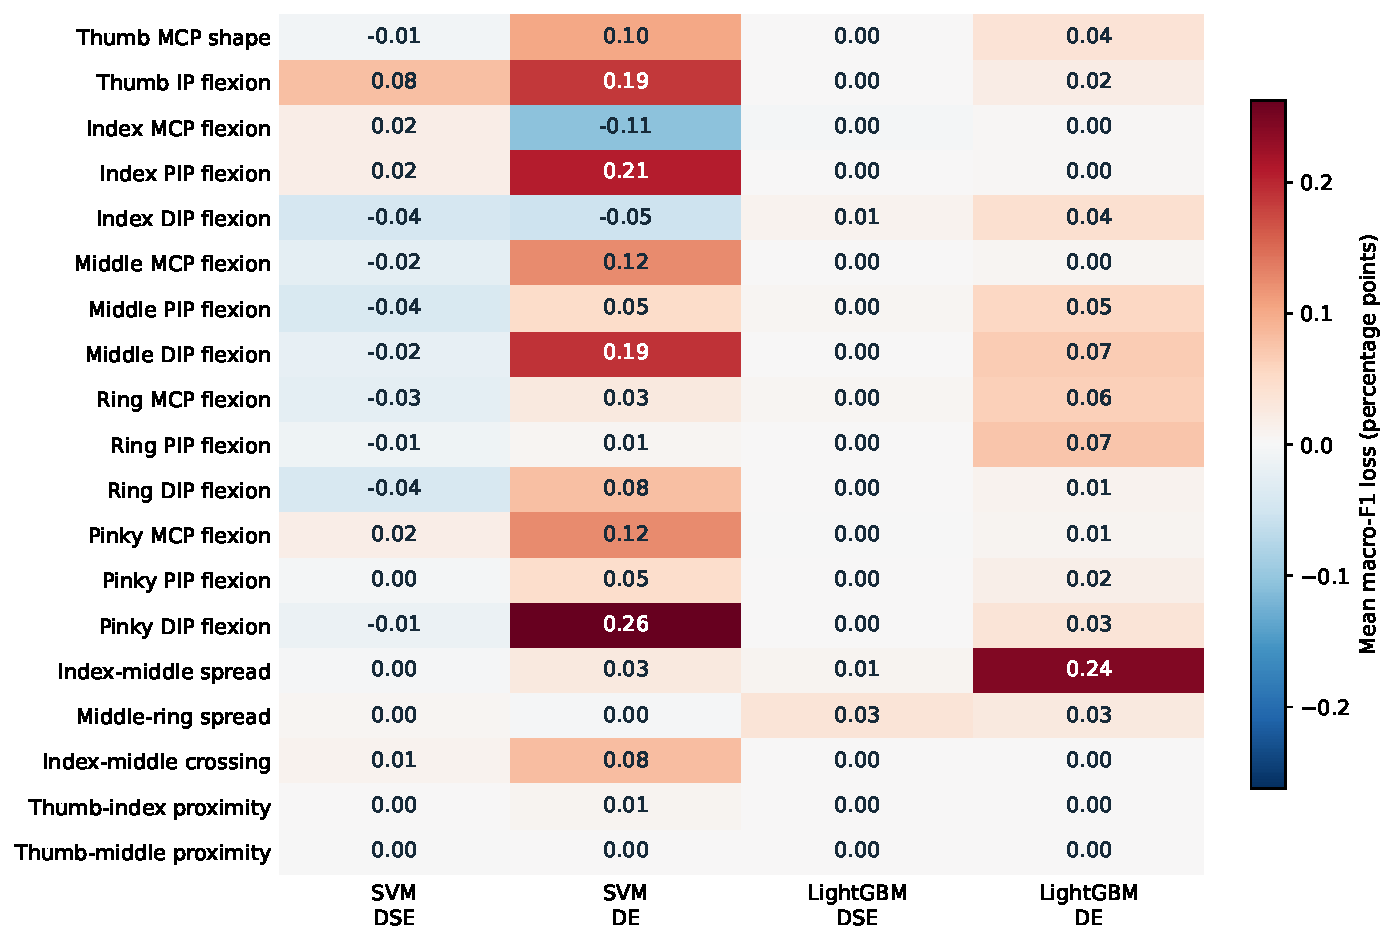
\includegraphics[width=.95\linewidth]{figures/ton_category_importance_en.pdf}
\caption{The 19 own checks, with all one-hot columns of a check shuffled together. Values are mean macro-F1 losses in percentage points over five folds and five shuffles. DSE contains Shin's directions; DE omits them. J is absent in both. Negative losses are retained.}
\label{fig:ton-permutation}
\end{figure}

In DSE, thumb IP flexion has the largest mean F1 loss among E checks for SVM (0.08 percentage points); middle--ring spreading is largest for LightGBM (0.03). These describe fitted-model dependence, not a guaranteed gain from adding a check.

Reproduce with \texttt{python -m RQ3 features} and \texttt{python -m RQ3 coordinate\_control}; commands and output directories are defined in \path{RQ3/workflows.py}. Feature definitions are in \path{research/feature_study.py}; evidence is in \path{results/feature_factorial_01/}. The protocol, 80 fold models, predictions, paired changes, controls, permutation outputs and verification preserve all values underlying the main table. The optional optimized SVM replay checks its outputs against ordinary SVC predictions; it does not alter the experiment.

\clearpage
\section{Own hand features and the inspection tool}\label{app:ton-tool}
The 19 checks comprise 13 flexion checks, two spreading checks, one crossing check, one thumb-shape check and two thumb-tip proximity checks. Multiple categories produce 70 one-hot inputs. They describe estimated landmarks, not independently verified anatomy.

\begin{figure}[h]\centering
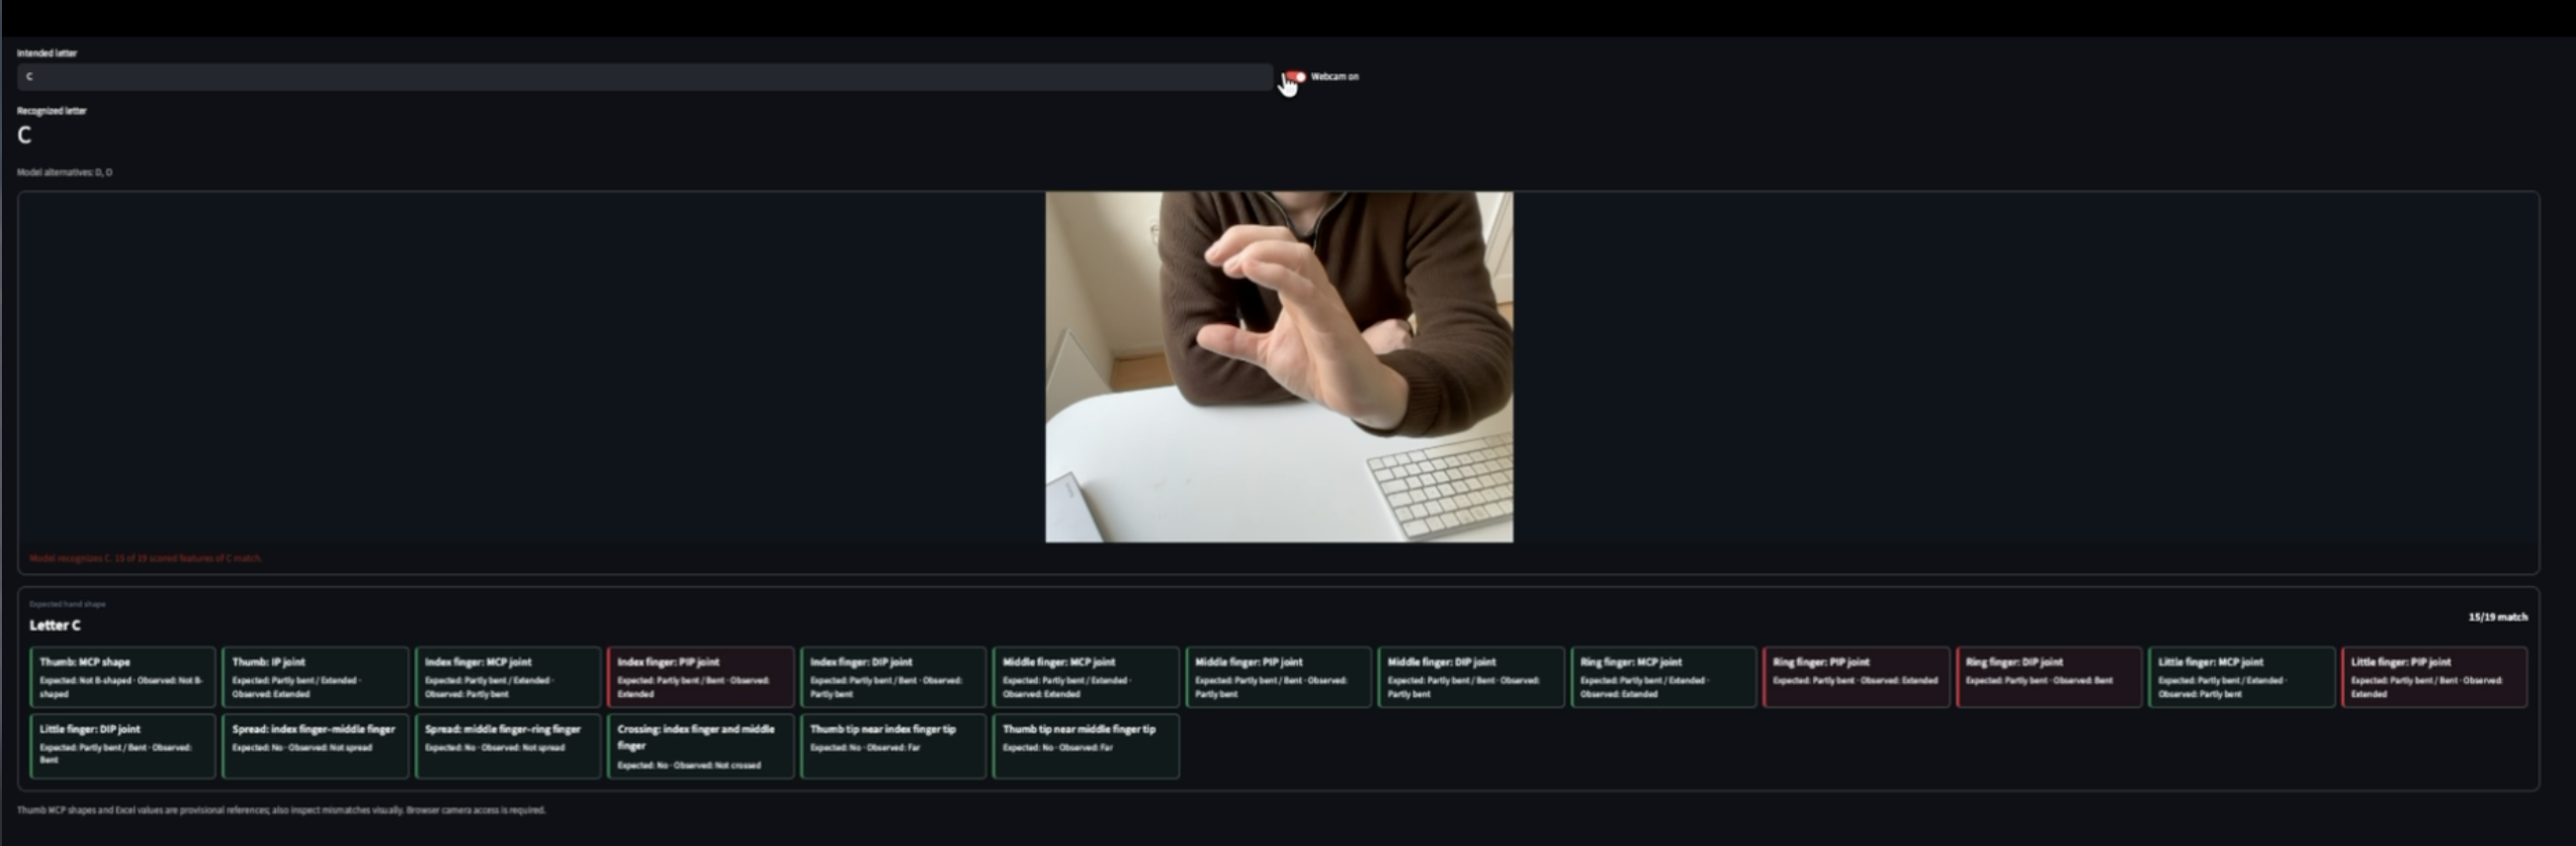
\includegraphics[width=.98\linewidth]{figures/ton_feature_tool_screenshot.png}
\caption{User-supplied feature-tool screenshot. Intended and predicted letter are both C, while only 15 of 19 workbook checks match. The target letter selects expected categories; it does not enter the classifier. Green/red cards indicate agreement with the chosen rules, not confidence in the predicted letter.}
\label{fig:ton-tool}
\end{figure}

\begin{table}[h]\centering\small
\caption{Own feature ideas and their implemented approximations. Thresholds are project choices, stored in \texttt{config/thresholds.json}.}
\begin{tabular}{p{.20\linewidth}p{.70\linewidth}}\toprule
Feature & Measurement and interpretation\\\midrule
Finger flexion (13) & Thumb IP and MCP/PIP/DIP of the other four fingers. A straight joint approaches $180^\circ$. Bent at at most $130^\circ$, extended from $150^\circ$, partly bent between these. Thumb IP uses $80^\circ$ and $155^\circ$.\\
Spreading (2) & Index--middle and middle--ring evaluated separately: normalized lateral gap at least 0.25, depth gap at most 0.6, positive direction cosine, and PIP/DIP angles at least $120^\circ$.\\
Crossing (1) & Index and middle reverse lateral order along their finger profiles, with depth difference at most 0.7 and sufficient extension. Crossing lines in 2D alone are insufficient.\\
Thumb shape (1) & The idea of the thumb across versus beside the palm is approximated by signed thumb-MCP deviation: B-shaped above $16^\circ$ towards the palm. This does not directly measure palm coverage.\\
Thumb-tip proximity (2) & Separate distances to index and middle tips, divided by wrist--middle-MCP length: contact at most 0.1; near up to 0.825; far above this.\\\bottomrule
\end{tabular}
\end{table}

MCP denotes the knuckle, PIP the middle joint, and DIP the end joint; the thumb has an IP joint. The measurements use estimated 3D world points. ``Not spread'' is not the same as touching: the pair can be adjacent, bent or crossed. Direct contact is only checked for the two thumb-tip pairs. ``Not B-shaped'' includes several thumb positions.

The workbook can allow several categories per letter. For ``no contact'', both near and far count as agreement. Unknown measurements are not confirmed agreement; blank reference fields are not scored. In the screenshot, index PIP is observed extended although partly bent/bent is expected, while index--middle is correctly observed not spread. The original screenshot is retained unchanged. The live tool also preserves the actual image, model hash, features and prediction for error analysis.

\clearpage
\section{Exploratory orientation follow-ups}\label{app:ton-orientation}
These short practical explorations tried left/right handling and G/H orientation alongside the main feature study. They retain their own 835-input SVM reference (DSJ) and are not extra arms of the eight-way comparison or independent final validation. The detail below makes the attempted ideas reproducible.

\subsection{RGB mirrors and detector-Right normalization}
Original and horizontally mirrored RGB images are independently detected with IMAGE mode, at most two hands, and detection/presence thresholds 0.5. There are 60,251 accepted originals and 60,201 accepted mirrors. Mirror training adds accepted mirrors of fitting sources while retaining total weight one per source. Original-only preprocessing, numeric gamma and class weights are shared. Sources and their copies remain in the same fold.

Normalization instead uses each detection's own hand label: detector-Left image points receive $x'=1-x$, world points $x'=-x$, then the hand label becomes Right. Other coordinates and anatomical indices remain unchanged; features are recomputed before fitting and inference. This reflection is not a palm-to-back rotation. Detector-Right is unchanged; unknown labels are rejected.

The fixed artificial mixture selects half the source images per letter/fold for RGB mirroring, using seed 20261106 before checking detection success. It contains 60,225 accepted images. Within each presentation all models use the same accepted sources; failed detections are excluded. This is not a verified equal mixture of real left- and right-handed users.

\begin{table}[h]\centering\small
\caption{SVM orientation checks: accepted detections only. P is macro-precision (\%); each test presentation has its own denominator.}
\begin{tabular}{llrrrr}\toprule
Test presentation & Training/input & N & P & Macro-F1 & Correct\\\midrule
\tonTableInput ton_orientation_rows_en.tex
\bottomrule\end{tabular}
\end{table}

On original images, normalization loses 136 correct predictions relative to no change, and mirror training loses 26. On the artificial mixture, normalization improves on no change but remains below mirror training. Detector labels are not independently verified; mirror pairs share pose, person and background. These results do not establish performance for unseen left-handed people. Evidence: \path{results/mirror_01/} and \path{results/handedness_01/}.

\subsection{Why G/H rotation is a different hypothesis}
For usual ASL G/H, the palm faces inward or sideways \citep{ton-vicarsfeedback}. Selected Kaggle training examples show the palm towards the camera. This motivates a possible training/use mismatch, not a demonstrated fault in Shin's learning method; all labels and camera viewpoints have not been independently checked.

A $180^\circ$ camera-$y$ rotation maps wrist-relative coordinates $(x,y,z)$ to $(-x,y,-z)$, with determinant $+1$. Horizontal reflection instead changes only $x$ and has determinant $-1$. A rotated G/H fitting copy and its original each weigh 0.5; other sources retain weight one. The 4,801 G/H sources yield 65,052 fitting rows in the full-data fit. The rotation preserves distances and intrinsic joint measurements; it produces no new RGB image or detector output.

\clearpage
\section{Exploratory G/H checks: artificial versus live views}\label{app:ton-live}
The first test retains all 60,251 accepted original images, including palm-facing G/H labels. The separate artificial control rotates only the 4,801 held-out G/H descriptions; other letters retain their original predictions. Models are not refitted for this test. Neither test independently validates ASL execution. Recognizing an atypical palm-facing G/H is not the intended live-use goal.

\begin{table}[h]\centering\small
\caption{G/H rotation checks over all 26 letters. Both presentations use the same 60,251 sources, but the artificial test replaces G/H geometry.}
\begin{tabular}{llrrr}\toprule
Test descriptions & Training & P (\%) & Macro-F1 & Correct\\\midrule
\tonTableInput ton_gh_rows_en.tex
\bottomrule\end{tabular}
\end{table}

Rotation corrects four original-view errors and introduces five (net $-1$). On the artificial control, it corrects 4,776 errors and loses three (net +4,773); G/H recall reaches 99.47\%/99.45\%. The added geometry is learned, but this is not real hand-back detection. Evidence: \path{results/rotation_GH_y180_01/} and \path{results/gh_occlusion_01/}.

\subsection{Exploratory approximation of occlusion}
A coarse palm ellipsoid and finger volumes are built around source landmarks and rendered with a depth buffer. MediaPipe accepts 64/64 original photographs but 0/64 renders at either 0 or 180 degrees (0/128 total). This rendering route supplies no training detections; known source points are not substituted for failed detector output.

A separate proxy rotates image/world landmarks and adds reproducible Gaussian coordinate noise only to finger joints hidden behind another estimated hand component. The two fixed standard deviations are 2\% and 5\% of wrist--middle-MCP length, scaled separately for image/world coordinates. All 835 features are recomputed. Original fitting weights, folds, preprocessing, gamma and class priors remain fixed. Ten new fold models give no extra gain over pure rotation on either the original or clean artificially rotated test. This is assumed point uncertainty, not a measured distribution of MediaPipe occlusion errors. No independent real hand-back evaluation is implied.

\clearpage
\subsection{Four user-selected live examples}
The original stored landmarks, without redetection, are replayed through both frozen deployment models. All four are accepted detections; model hashes, stored input vectors and recorded predictions are checked. Both hand-back G examples remain H after rotation training. An H changes from Z to H, and a G with the palm visible remains G. Intended letters are user annotations and views are described visually, not expert ASL ground truth. The examples are selected error analysis, not a frequency or accuracy estimate.

\begin{figure}[h]\centering
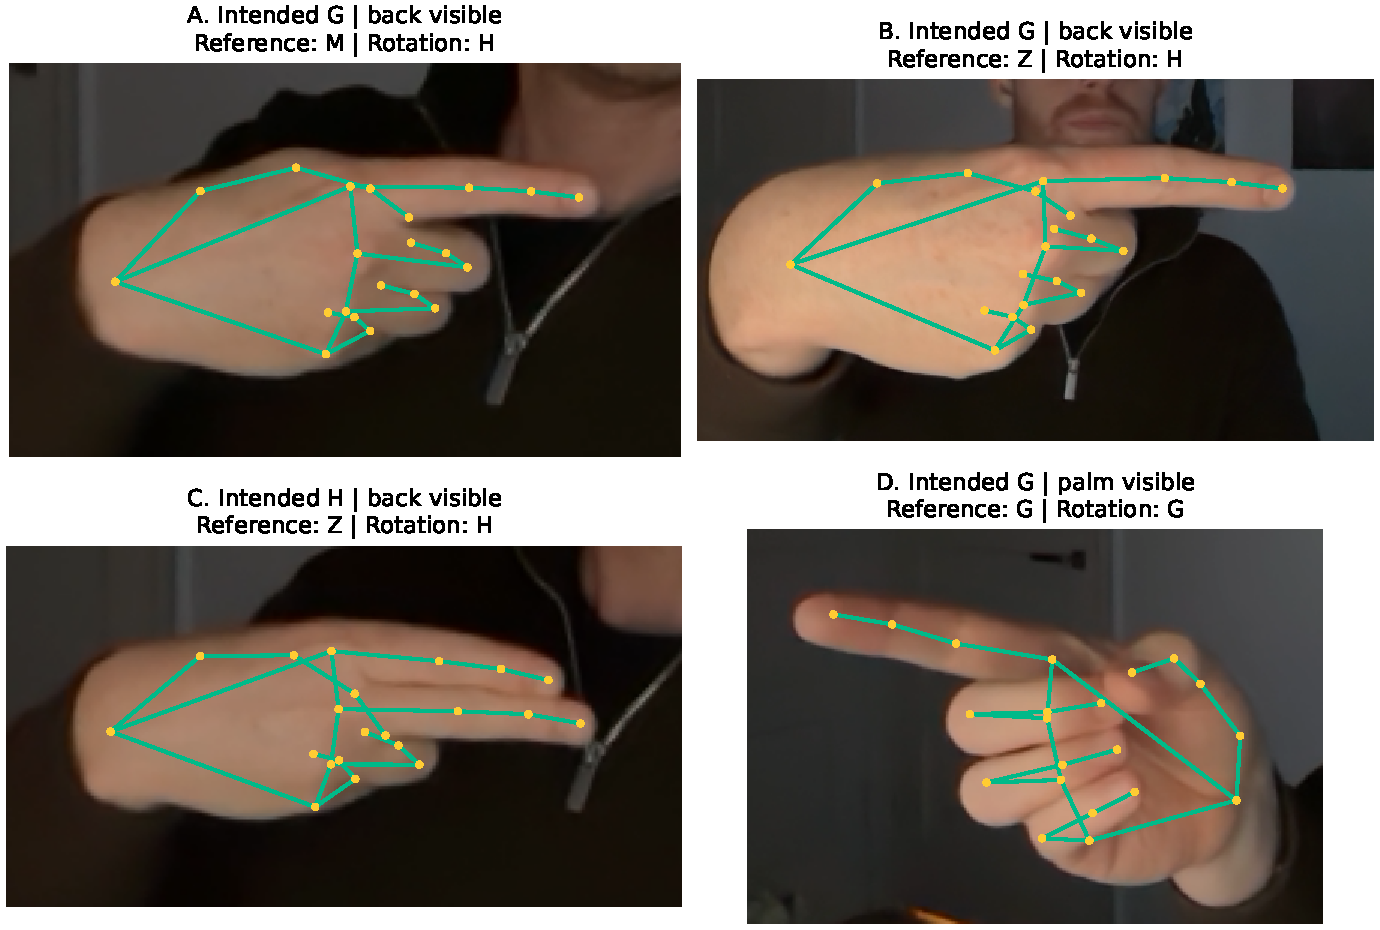
\includegraphics[width=.74\linewidth]{figures/ton_live_examples_en.pdf}
\caption{All four new live examples with stored landmarks. A/B: intended G remains H; C: H is recovered; D: G is recognized with the palm visible. ``Reference'' and ``Rotation'' are model outputs. No image is used for training.}
\label{fig:ton-live}
\end{figure}

The middle-finger DIP estimates in A/B are 161.7 and 164.7 degrees, compared with a G-training median of 113.2 (middle 50\%: 109.2--118.2). Signed thumb deviation is $-1.9$ and $2.7$ degrees versus median 35.9. These are estimated world-point measurements, not true 3D anatomy. Pose, viewpoint and detector error cannot be separated here, nor is one angle proven to cause the classifier error. A rigid rotation preserves the original joint geometry and does not recreate such new detection changes.

The high artificial score therefore does not directly transfer to the live camera. Rotation training is not yet a demonstrated solution to the observed G/H confusion. This observation does not establish the general failure rate. Source IDs, paired outputs, measurements and hashes: \path{results/gh_live_diagnostics_20261107/}.


\end{document}

